\chapter{Metodologia}

\section{Introducción}
Se eligió la metodología \textbf{SCRUM} dado que es una de las más utilizadas a nivel empresarial y con ella se puede llegar a entregar un producto de calidad optimizando el tiempo de desarrollo, además de esto, es importante resaltar que hace el uso de un concepto propio como es del sprint, el cual es una carrera corta o se podría ver como un subproceso, y consideramos que es importante dividir un proceso en subprocesos para poder llevar a cabo correctamente una dinámica colaborativa para obtener buenos resultados con calidad y agilidad.\\
En la fase In-Game, se decidió utilizar el proceso en cascada dado que es simple y lineal, es decir que cada una de las etapas se complementa de la anterior para poder cumplir su funcionalidad dentro del modelo, además de esto, es importante resaltar la parte de la documentación en este proceso dado que en cada etapa se producen informes con el fin de hacer que la comprensión del procedimiento del producto a diseñar sea más sencillo. Además de esto el modelo en cascada posee una gran ventaja como lo es la planificación fácil y clara por parte de los desarrolladores y el usuario, y para complementar la fase de implementación de cascada se utilizará el proceso de Codificación y Reparación. \\

\begin{figure}[H]
	\centering
	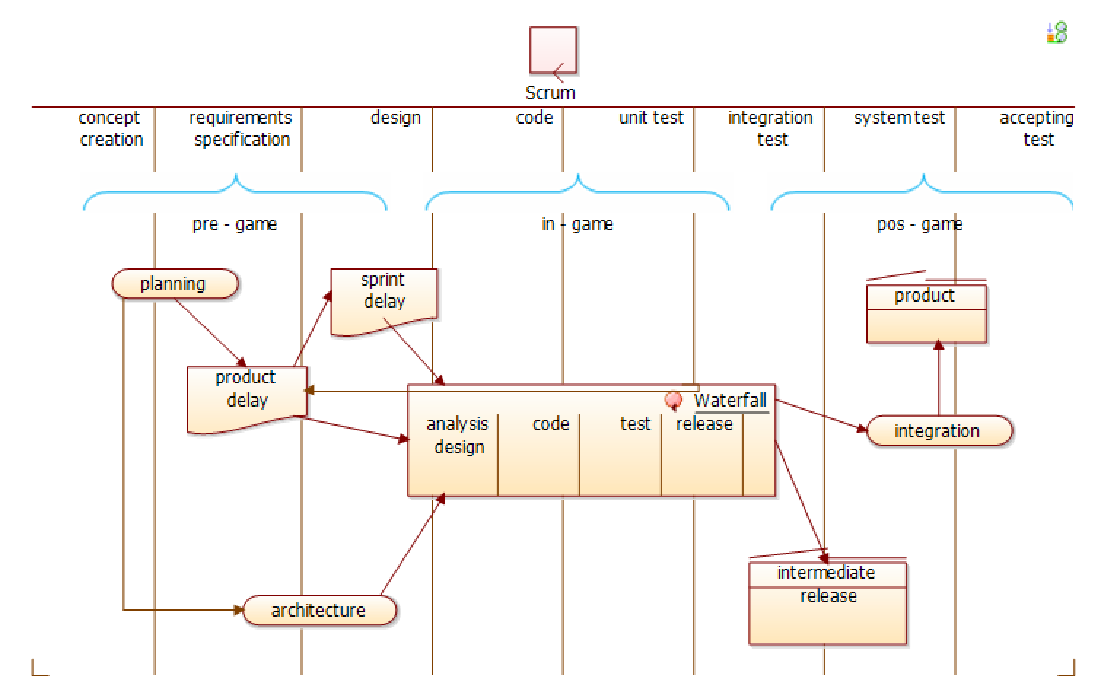
\includegraphics[scale=0.65,]{imagenes/Metodologia/Scrum.pdf}
	\caption{Metodología Scrum.}
	\label{fig:cronograma}
\end{figure}

Haciendo énfasis en todo lo que conlleva hacer uso de esta metodología para el desarrollo de nuestro proyecto, de debe hablar de que se realizará en cada una de las etapas planteadas en esta metodología, también se mostrará el cronograma relacionado con esta metodología y los procesos a utilizar, pero primero que todo se definirá el Scrum Master y Team Members.\\

\textbf{Scrum Master}: La persona encargada de cumplir las tareas de un Scrum Master será \textit{Johan Quiroga}, ya que dadas sus cualidades califica perfectamente para llevar a cabo este cargo, además tiene un perfil de un líder dado que supervisará, verificará y será el facilitador del equipo de trabajo.\\

\textbf{Team members}: las personas que conformarán el Team Members serán \textit{Daniela Cordoba} y \textit{Santiago Jimenez} quienes se enfocaran en las tareas de desarrollo del software y los cuales tienen las capacidades técnicas para poder desarrollar el producto a cabalidad.\\

\textbf{Planeación del Sprint}: En este proceso el \textit{Scrum Master} y el \textit{Team Members} se reunirán para planear las actividades que se encuentran inmersas dentro del sprint a realizar es decir se deben dar prioridad dentro de estas actividades y dar todas la información pertinente como lo es el tiempo disponible para esta iteración obteniendo así referencias para el próximo sprint.\\

\textbf{Reunión diaria de Scrum}: En cuanto a las reuniones diarias en este proyecto cambiaremos un poco ese concepto dado que aunque se realizarán diariamente, no al inicio del día, sino que por el contrario se hará una reunión finalizando el día para saber que los miembros que participan en estas reuniones puedan hacer y responder preguntas como ¿Qué se hizo durante el día?, ¿Qué se planea hacer el día siguiente? Y saber si se ha presentado algún tipo de inconveniente en el proceso de alcanzar el objetivo además estas reuniones tendrán un intervalo de durabilidad de entre unos 15 a 20 minutos diarios.\\

\textbf{Revisión del sprint}: Cada vez que se dé por terminado un sprint se debe mostrar lo que el equipo ha logrado, es decir un producto terminado referente a ese sprint que se estaba trabajando para saber si esta óptimo o si se deben hacer algunas correcciones esto se analizará dentro del grupo de trabajo y el dueño del producto, aclarando que los sprints serán realizados con las características de el proceso en Cascada.

\section{Scrum/Cascada/Codificación y Reparación}

\subsection{Pre-Game}
En esta sección se  especificará que se hará durante las dos fases que la componen como lo son la planeación y la escenificación.

\subsubsection{Planeación (Planning)}
Durante este segmento o fase se realiza una reunión entre todos los entes involucrados en el desarrollo de este proyecto como lo son the power owner, scrum master y team members  para poder definir la visión, la expectativas y el presupuesto con el que se cuenta para el desarrollo de este además de esto the power owner debe de lanzar la pila de producto que contengan los elementos suficientes para poder entrar a un primer sprint.

\subsubsection{Staging (Escenificación)}
Durante esta fase se tomara en cuenta lo especificado o planteado en la fase anterior es decir en la fase de planeación dado que se tiene que tener claro el presupuesto y los requisitos planteados, es importante traer de la fase de planeación la lista de producto dado que por medio de esta se llegará al planteamiento de los requerimientos los cuales son de suma importancia para el desarrollo de nuestro proyecto. En esta fase se verán involucrado tanto el \textit{Scrum Master} como el \textit{Team Members} dado que entre ellos se analizará la lista de producto para poder llegar a unos requerimientos que satisfagan el proyecto.

\subsection{In-Game}
En esta sección se  especifica la duración de cada uno de los sprints por medio de el procesos cascada a el cual se le ha integrado el proceso de codificación y reparación.
\subsubsection{Proceso en Cascada (Waterfall)}
\begin{figure}[H]
	\centering
	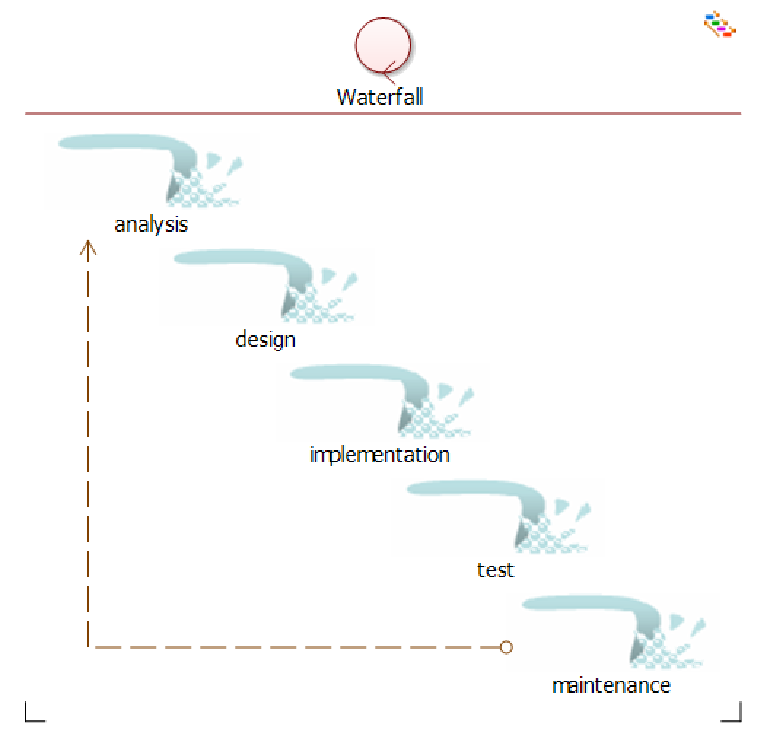
\includegraphics[scale=0.7,]{imagenes/Metodologia/Waterfall.pdf}
	\caption{Proceso Waterfall}
	\label{fig:cronograma}
\end{figure}

\paragraph{Análisis (Analysis)}
Durante esta etapa se tendrán en cuenta los requisitos del sistema planteados por el cliente. Además de esto una parte importante de esta etapa hace referencia al desarrollo de cada uno de los requerimientos, es decir que a través de la información suministrada por el cliente se plantearán cada uno de los requerimientos y se desarrollará la interacción, es decir los casos de uso, casos de secuencia, casos de comunicación y workflow, para así tener planteamientos específicos, concretos y sin lugar a ambigüedades.

\paragraph{Diseño (Design)}
Luego de finalizada la etapa de análisis se tomarán los desarrollos realizados en requerimientos e interacciones, ya que por medio de ellos se planteará un diseño que le brinde solución a la situación problema planteada por el cliente, es así como se tomará cada uno de los requerimientos y se les aplicará este mismo proceso de diseño y solución para poder pasar a la siguiente etapa la cual es la de implementación y poder facilitar este proceso por medio de un diseño claro y conciso.

\paragraph{Implementación (Implementation)}
En esta etapa se hará uso de un nuevo proceso el cual es CODIFICACIÓN Y REPARACIÓN con el cual se busca utilizar cada uno de los diseños o soluciones planteadas y por medio de algoritmia o codificación poder plasmar estas soluciones a nivel de código.

\subparagraph{Codificación y Reparación}
Se utilizará el proceso de codificación y reparación dado que es un modelo simple que está orientado a la parte de desarrollo, pues que encaja perfectamente dentro de la etapa de implementación dentro de la cual se encuentra inmersa, a pesar de que no está compuesta por una etapa de prueba, y es un buen complemento para el correcto y efectivo desarrollo de la codificación.
%imageeeeeeeeeeeeeeeeeeeeeen
\begin{figure}[H]
	\centering
	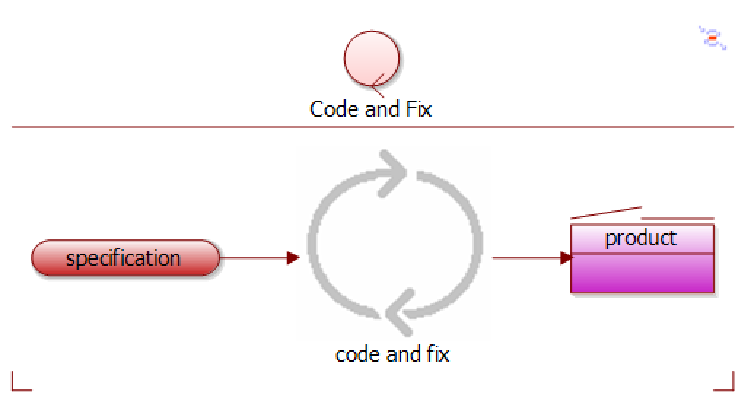
\includegraphics[scale=0.9,]{imagenes/Metodologia/Code-and-fix}
	\caption{Proceso Code and Fix}
	\label{fig:cronograma}
\end{figure}

\subsubparagraph{Especificación}
En esta etapa se hará uso de los requerimientos y los diseños planteados en la etapa de análisis y diseño del proceso en cascada los cuales se analizarán para poder seguir adelante en este proceso y llevar esto a la siguiente etapa la cual es Codificación y Reparación.

\subsubparagraph{Codificación y Reparación}
Durante esta etapa se realizan constantemente ciclos en los cuales se hará uso de esa especificación ya realizada anteriormente para poder tomar cada diseño o solución planteada y así poder traducir esto a un lenguaje que la maquina entienda.

\subsubparagraph{Producto}
Después de dar como finalizada la etapa anterior en esta fase se tendrá el producto final, el cual en este caso será la implementación de un diseño y una solución en particular para que de esta manera sea posible abarcar en su totalidad todas los diseños de  las soluciones planteadas.

\paragraph{Prueba (Test)}
Luego del desarrollo de las soluciones de diseño y su implementación se realizaran pruebas necesarias para poder verificar que nuestro producto final tenga la calidad necesaria para que la cantidad de errores sea mínima con el objetivo de reducir el tiempo de trabajo en la etapa de mantenimiento, además de esto se harán uso de ciertas pruebas como lo son:
\begin{itemize}
	\item Prueba unitaria.
	\item Prueba de integración.
	\item Pruebas del sistema.
	\item Prueba de aceptación.
\end{itemize}


\paragraph{Mantenimiento (Maintenance)}
En este caso enfocaremos esta etapa a la corrección de los errores encontrados en el producto final, en un dado caso que en la etapa anterior se presente algún tipo de error, se manejará un mantenimiento preventivo y perfectivo dado que por medio este se busca prever posibles errores a futuro direccionándonos a obtener un producto de una muy buena calidad que satisfaga las necesidades del cliente propuestas en la etapa de análisis con un mínimo de requisitos de hardware.


\subsection{Post-Game}
En esta sección se  especificarán las partes que componen esta fase como lo es el release o liberación.

\subsubsection{Release (Liberación)}
En esta etapa se busca dar y entregar el producto final utilizando conjuntamente el concepto de integración, dado que se utilizara para poder unir los subsistemas creados en el in-game y por medio de este término poder integrarlos y unirlos para tener un producto final integrado y finalizado cumpliendo exitosamente lo propuesto al inicio de nuestro proyecto.


\section{Cronograma}
Cabe resaltar que el cronograma planteado está directamente relacionado con nuestro desarrollo de software el cual incluye la metodología Scrum y los procesos en Cascada y, codificación y reparación.

%%%imageeeeen cronograma
%\includegraphics{imagenes/imgs/cronograma}
\begin{figure}[H]
	\centering
	\includegraphics[scale=0.10,]{imagenes/Metodologia/cronograma.pdf}
	\caption{Cronograma de metodología Scrum }
	\label{fig:cronograma}
\end{figure}

\subsection{Pre-Game}
Esta fase tiene una duración de 16 días, en los cuales se buscara cumplir cada una de las funciones que tienen cada una de las etapas que componen el pre-game estos días están distribuidos de la siguiente forma:
\begin{itemize}
	\item \textbf{Planificación}: esta etapa abarca un total de 8 días en los cuales se buscara cumplir la meta propuesta anteriormente.
	\item \textbf{Escenificación}: esta etapa cuenta con  un total de 8 días en los cuales se buscara cumplir las tareas propuestas anteriormente.
	
\end{itemize}

Dentro de esta fase podemos encontrar un primer sprint el cual se desarrollara durante la etapa de escenificación.

\subsection{In-Game}
Esta fase tiene una duración de 60 días en los cuales se buscara cumplir cada una de las funciones que tienen cada una de las etapas que componen el pre-game y estos días están distribuidos de la siguiente forma con el uso de los procesos mencionados anteriormente:

\subsubsection{Cascada}
\begin{itemize}
	\item \textbf{Análisis}: esta etapa cuenta con  un total de 10 días en los cuales se buscará cumplir y analizar lo propuesto en la escenificación y la codificación.
	\item \textbf{Diseño}: esta etapa abarca un total de 30 días en los cuales se buscará cumplir con los diseños de software.
	\item \textbf{Implementación}: esta etapa abarca un total de 18 días en los cuales se usará el proceso de Codificación y Reparacion para llevar acabo el desarrollo de esta.
	\item \textbf{Prueba}: esta etapa no cuenta con días en el calendario dado que no se llegará a esta.
	\item \textbf{Mantenimiento}: al igual que en la etapa de prueba, no se realizará dado que no se llegará a ese punto.
	
	
	
	
\end{itemize}

Dentro de esta fase encontramos 3 sprints de tipo macro ubicado en cada una de la etapas como lo son las rápidas cascadas que se realizaran y cada uno de esos macro-sprint se componen por varios micro-sprint los cuales son el proceso de Codificación y Reparación, esto está relacionado con el número de requerimientos los cuales se pondrán a ser procesados en cada una de estas etapas.

\subsection{Post-Game}
Esta fase tiene una duración de 6 días en los cuales se buscará cumplir cada una de las funciones que tiene la liberación:
\begin{itemize}
	\item \textbf{Liberación}: esta etapa cuenta con un total de 6 días en los cuales se entregará el producto.
\end{itemize}
	

